\begin{enumerate}
  \item Remove harmonics
  \item Sync re-sample
  \item Filter
  \item Can also average many traces
  \item \ldots
\end{enumerate}

The first step in the signal processing was to isolate the information bearing signal. The most straightforward step was hence to remove the 4MHz signal and its harmonics that arise from the main processor. The 30.8 GHz signal we are interested in is preserved as shown in Figure \ref{figure:harmonics_removal}.

    \begin{figure*}
      \centering
      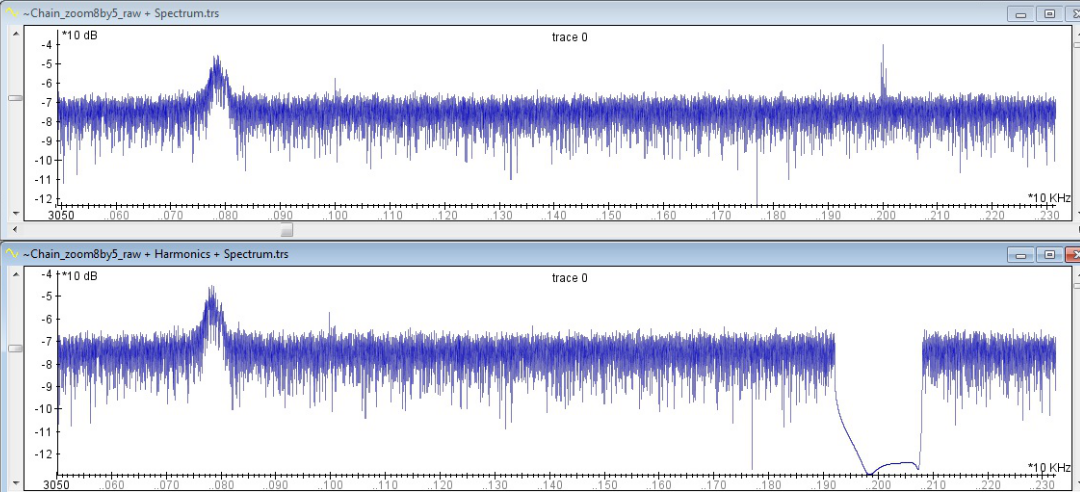
\includegraphics[scale=0.38]{img/harmonics_removal.png}
      \caption{\label{figure:harmonics_removal}Removal of 4GHz harmonics.}
    \end{figure*}  

The next step was to resample the original signal at a 30.8 GHz sample rate.
